%%%%%%%%%%%%%%%%%%%%%%%%%%%%%%%%%%%%%%%%%
% Beamer Presentation
% LaTeX Template
% Version 1.0 (10/11/12)
%
% This template has been downloaded from:
% http://www.LaTeXTemplates.com
%
% License:
% CC BY-NC-SA 3.0 (http://creativecommons.org/licenses/by-nc-sa/3.0/)
%
%%%%%%%%%%%%%%%%%%%%%%%%%%%%%%%%%%%%%%%%%

%----------------------------------------------------------------------------------------
%	PACKAGES AND THEMES
%---------------------------------------------------------------------------------------

\documentclass{beamer}
\usepackage[spanish]{babel}
\usepackage{algpseudocode}
\usepackage[utf8]{inputenc}
\mode<presentation> {

% The Beamer class comes with a number of default slide themes
% which change the colors and layouts of slides. Below this is a list
% of all the themes, uncomment each in turn to see what they look like.

%\usetheme{default}
%\usetheme{AnnArbor}
%\usetheme{Antibes}
%\usetheme{Bergen}
%\usetheme{Berkeley}
%\usetheme{Berlin}
%\usetheme{Boadilla}
%\usetheme{CambridgeUS}
%\usetheme{Copenhagen}
%\usetheme{Darmstadt}
%\usetheme{Dresden}
%\usetheme{Frankfurt}
%\usetheme{Goettingen}
%\usetheme{Hannover}
%\usetheme{Ilmenau}
%\usetheme{JuanLesPins}
%\usetheme{Luebeck}
%\usetheme{Madrid}
%\usetheme{Malmoe}
%\usetheme{Marburg}
%\usetheme{Montpellier}
\usetheme{PaloAlto}
%\usetheme{Pittsburgh}
%\usetheme{Rochester}
%\usetheme{Singapore}
%\usetheme{Szeged}
%\usetheme{Warsaw}

% As well as themes, the Beamer class has a number of color themes
% for any slide theme. Uncomment each of these in turn to see how it
% changes the colors of your current slide theme.

%\usecolortheme{albatross}
%\usecolortheme{beaver}
%\usecolortheme{beetle}
%\usecolortheme{crane}
%\usecolortheme{dolphin}
%\usecolortheme{dove}
%\usecolortheme{fly}
%\usecolortheme{lily}
%\usecolortheme{orchid}
%\usecolortheme{rose}
%\usecolortheme{seagull}
%\usecolortheme{seahorse}
%\usecolortheme{whale}
%\usecolortheme{wolverine}

%\setbeamertemplate{footline} % To remove the footer line in all slides uncomment this line
%\setbeamertemplate{footline}[page number] % To replace the footer line in all slides with a simple slide count uncomment this line

%\setbeamertemplate{navigation symbols}{} % To remove the navigation symbols from the bottom of all slides uncomment this line
}

\usepackage{graphicx} % Allows including images
\usepackage{booktabs} % Allows the use of \toprule, \midrule and \bottomrule in tables

%----------------------------------------------------------------------------------------
%	TITLE PAGE
%----------------------------------------------------------------------------------------

\title[Practica 3]{Greedy:\\
Travelling Salesman Problem} % The short title appears at the bottom of every slide, the full title is only on the title page

\author{Algorítmica} % Your name
\institute[UGR] % Your institution as it will appear on the bottom of every slide, may be shorthand to save space
{
Universidad de Granada \\ % Your institution for the title page
\medskip

}
\date{\today} % Date, can be changed to a custom date

\begin{document}

\begin{frame}
\titlepage % Print the title page as the first slide
\end{frame}

\begin{frame}
\frametitle{Índice} % Table of contents slide, comment this block out to remove it
\tableofcontents % Throughout your presentation, if you choose to use \section{} and \subsection{} commands, these will automatically be printed on this slide as an overview of your presentation
\end{frame}

%----------------------------------------------------------------------------------------
%	PRESENTATION SLIDES
%----------------------------------------------------------------------------------------

\section{Introducción }
\begin{frame}
	\frametitle{Introducción}
	\begin{itemize}
		\item El objetivo de esta práctica es diseñar varios algoritmos Greedy resolviendo el problema del viajante de comercio o TSP
	\end{itemize}
\end{frame}


%------------------------------------------------
\section{Primera versión} 
\begin{frame}
	\frametitle{Primera versión}
	Aplicar algoritmo usando Greedy simple, buscaremos en cada momento la ciudad más cercana y esa ciudad
	la añadiremos a nuestro conjunto de soluciones. 
	
\end{frame}

%------------------------------------------------
\subsection{Diseño del algoritmo} 
\begin{frame}
	\frametitle{Diseño del algoritmo}
	\begin{itemize}
		\item \textbf{Conjunto de candidatos}: Conjunto de ciudades. (Conjunto \textbf{C})
		\item \textbf{Conjunto de seleccionados}: Conjunto de ciudades ordenado. (Conjunto \textbf{S})
		\item \textbf{Función solución}: Cuando el conjunto de candidatos esté vacío.
		\item \textbf{Función factibilidad:} Cuando la ciudad no ha sido visitada.
		\item \textbf{Función selección}: Se seleccionará la ciudad más cercana.
		\item \textbf{Función objetivo}: Lista con las ciudades en el orden en el que hay que visitarlas.		
	\end{itemize}
	
\end{frame}

\subsection{Pseudocodigo}
\begin{frame}
	\frametitle{Pseudocódigo I}
	Selección

	\begin{algorithmic}
	\Require Conjunto de ciudades C,S
	\State {x=0}
	\State {S=C[0]}
	\For {i = 1 to len(C)}
		\If{ C[i] MenorDistancia }
 	   		\State{x = C[i]}
 	   		\State{S.add(x)}
 	   		\State{C[i].erase}
		\EndIf
	\EndFor  
	
	\Return S	
	\end{algorithmic}	
\end{frame}


%------------------------------------------------
\section{Segunda versión} 
\begin{frame}
	\frametitle{Segunda versión}
	Aplicar algoritmo usando Greedy con selección parcial, estableceremos un recorrido inicial seleccionando las 3 ciudades más alejadas (oeste, norte y este). A partir de ahí añadiremos las ciudades con respecto a los intervalos creados.
	
\end{frame}

%------------------------------------------------
\subsection{Diseño del algoritmo} 
\begin{frame}
	\frametitle{Diseño del algoritmo}
	\begin{itemize}
		\item \textbf{Conjunto de candidatos}: Conjunto de ciudades. (Conjunto \textbf{C})
		\item \textbf{Conjunto de seleccionados}: Conjunto de ciudades ordenado. (Conjunto \textbf{S})
		\item \textbf{Función solución}: Cuando el conjunto de candidatos esté vacío.
		\item \textbf{Función factibilidad:} Cuando la ciudad no ha sido visitada.
		\item \textbf{Función selección}: Se seleccionará una ciudad y comprobaremos para cada una de las posiciones del circuito solución el mejor lugar para insertarlo (la que ofrece menor distancia) .
		\item \textbf{Función objetivo}: Lista con las ciudades en el orden en el que hay que visitarlas.		
	\end{itemize}
	
\end{frame}

\subsection{Pseudocódigo}
\begin{frame}
	\frametitle{Pseudocódigo I}
			\begin{algorithmic}				
						\Require Conjunto de ciudades C,S
						\State {x=0; S=CalcularRecorridoInicial();}
						\While {C}
							\For {i=0 to len(C)}
								\State{x = C[i];}
								\For{ j=1 to len(S-1)}
									\State {Saux = S; Saux[j] = x;}
									\If {distanciaSaux menor que minDistancia}
										\State {minDistancia = distanciaSaux;}
										\State {indiceSolucion = j; indiceCiudad = i;}
									\EndIf
								\EndFor
							\EndFor 
							\State{S[indiceSolucion] = x; C[indiceCiudad].erase;}
						\EndWhile 
						
						\Return S
					
			\end{algorithmic}

\end{frame}

\section{Tercera versión} 
\begin{frame}
	\frametitle{Tercera versión}
	Implementación del algoritmo Greedy 2-Opt. Calcularemos una primera aproximación de la solución utilizando el algoritmo de la primera versión. Después, iremos para cada ciudad intercambiando con las siguientes, viendo si alguno de esos intercambios mejora la primera solución obtenida, así hasta intentar generar una solución mejor que la primera
\end{frame}

%------------------------------------------------
\subsection{Diseño del algoritmo} 
\begin{frame}
	\frametitle{Diseño del algoritmo}
	\begin{itemize}
		\item \textbf{Conjunto de candidatos}: Conjunto de ciudades. (Conjunto \textbf{C})
		\item \textbf{Conjunto de seleccionados}: Conjunto de ciudades ordenado. (Conjunto \textbf{S})
		\item \textbf{Función solución}: Cuando el conjunto de candidatos esté vacío.
		\item \textbf{Función factibilidad:} Cuando la ciudad no ha sido visitada.
		\item \textbf{Función selección}: Dada la solución con la primera versión del algoritmo, comprobaremos si intercambiando una por una las ciudades se mejora la solución inicial.
		\item \textbf{Función objetivo}: Lista con las ciudades en el orden en el que hay que visitarlas.		
	\end{itemize}
	
\end{frame}

\subsection{Pseudocódigo}
\begin{frame}
	\frametitle{Pseudocódigo I}
	\begin{algorithmic}				
		\Require Conjunto de ciudades C,S,AUX
		\State S=PrimeraVersión();Z=Distancia(S);
		\State {x,y,i = 0; j = 1;}
		\While {\textbf{i} menor o igual \textbf{tam -2} and\textbf{ j} menor o igual a \textbf{tam - 1}}
			\State Sp=Swap(S,i,j);Zp=Distancia(Sp);
			\If {\textbf{Zp} mayor o igual que \textbf{Z} and \textbf{j} menor que \textbf{tam-1}}
				\State j++;
			\EndIf
			\If{\textbf{Zp} mayor o igual que \textbf{Z} and \textbf{j }== \textbf{tam - 1}}
				\State j++; i++;
			\EndIf
			\If {\textbf{Zp }menor que \textbf{Z}}
				\State S = Sp; Z = Zp;
				\State i++; j = i + 1;
			\EndIf
		\EndWhile  
		
		\Return S	
		
	\end{algorithmic}
	
	
\end{frame}

\section{Comparación}
\begin{frame}
	\frametitle{Comparación recorridos}
	En esta sección veremos los distintos resultados obtenidos de cada una de las ejecuciones de los algoritmos.
	
	\begin{table}[H]
		\centering
	
		
		\begin{tabular}{l|l|l|l|l}
			Mapa & Versión I & Versión II & Versión III  & Versión óptima  \\
			ulysses16 & 79.0141 & 81.1402 & 74.4295 & - \\
			berlin52 & 8314.81 & 9622.17 & 7883.92 & 7542  \\
			ch130 & 7022.12 & 7499.39 & 6738.84 & 6110 \\
			lin105 & 17173.4 & 19159.3 & 16139.2 & 14379 \\
			kroa100	& 25345.7 & 27646.1 & 24163.5 & 21282 \\
			pcb442 & 61536.8 & 61217.7 & 59520.4 & 50778 \\
		\end{tabular}
	
	\end{table}
	
\end{frame}


\begin{frame}
	\frametitle{Comparación gráficas}
	En esta sección veremos los distintos grafos obtenidos de cada uno de los algoritmos para el mapa Berlin52
	
	\begin{figure}
\centering
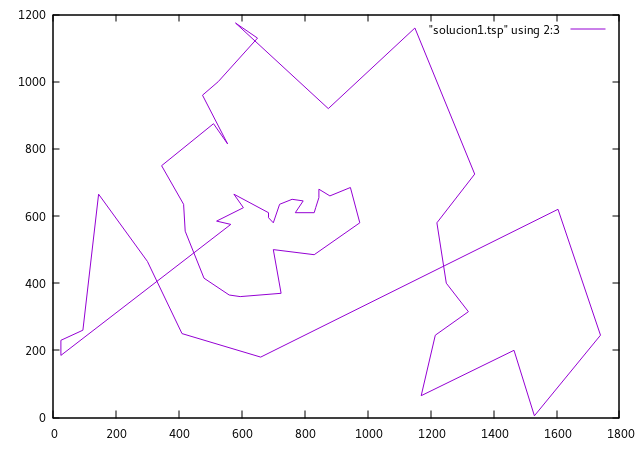
\includegraphics[width=0.7\linewidth]{../grafica/grafica1.png}
\caption{Primera versión}
\label{fig:graficafinal}
\end{figure}
	
\end{frame}
\begin{frame}
	\frametitle{Comparación gráficas}
	En esta sección veremos los distintos grafos obtenidos de cada uno de los algoritmos para el mapa Berlin52
	
	\begin{figure}
		\centering
		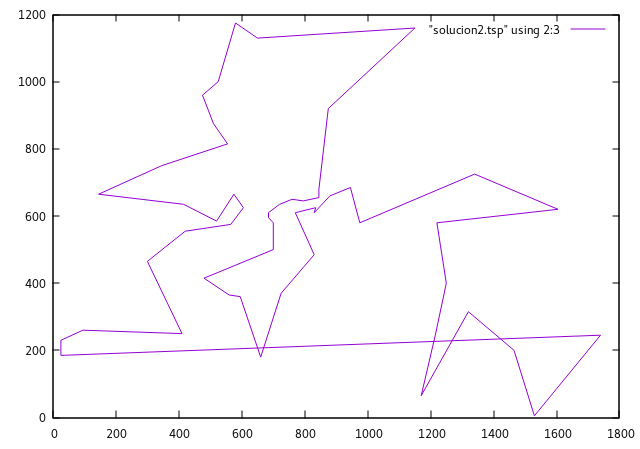
\includegraphics[width=0.7\linewidth]{../grafica/grafica2.png}
		\caption{Segunda versión}
		\label{fig:graficafinal}
	\end{figure}
	
	
	
\end{frame}
\begin{frame}
	\frametitle{Comparación gráficas}
	En esta sección veremos los distintos grafos obtenidos de cada uno de los algoritmos para el mapa Berlin52
	
	\begin{figure}
		\centering
		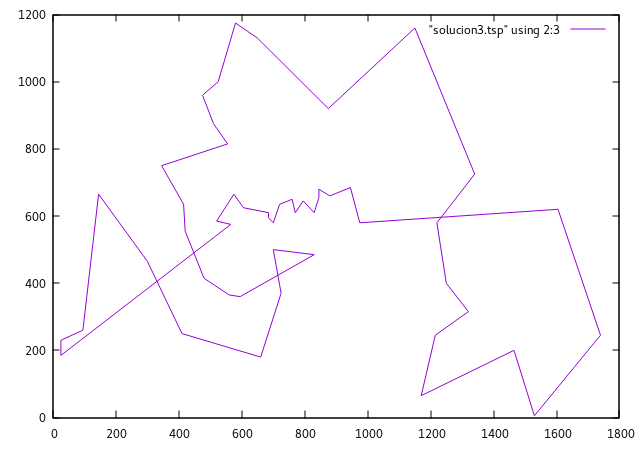
\includegraphics[width=0.7\linewidth]{../grafica/grafica3.png}
		\caption{Tercera versión}
		\label{fig:graficafinal}
	\end{figure}
	
	
	
\end{frame}






\end{document} 
